% !Mode:: "TeX:UTF-8" 
% !TEX program = xelatex
\documentclass[t,12pt,mathserif] {beamer} 

\usepackage[english]{babel}
\usepackage[utf8]{inputenc}
\usepackage[T1]{fontenc}
\usepackage{csquotes}
\usepackage{expl3,biblatex}
\usepackage{booktabs}
\usepackage{color,xcolor}
\usepackage{graphicx,caption,wrapfig,setspace}
\usepackage{amsthm,thmtools,amsmath,amsfonts,amssymb,dsfont} 
\usepackage{soul}
\usepackage{xeCJK}
\usepackage{newtxtext, newtxmath}

\usetheme{Madrid}
\usecolortheme{crane}
% set font
\usefonttheme{serif}

\definecolor{titlecolor}{RGB}{227, 169, 5}

\addtobeamertemplate{block begin}{%
  \setlength{\textwidth}{0.9\textwidth}%
}{}

\addtobeamertemplate{block alerted begin}{%
  \setlength{\textwidth}{0.9\textwidth}%
}{}

\addtobeamertemplate{block example begin}{%
  \setlength{\textwidth}{0.9\textwidth}%
}{}


\makeatletter
\let\HL\hl
\renewcommand\hl{%
  \let\set@color\beamerorig@set@color
  \let\reset@color\beamerorig@reset@color
  \HL}
\makeatother


\addbibresource{bibliography.bib}

% \usefonttheme[onlymath]{serif}
\mathversion{bold}
\setbeamerfont{normal text}{family=\sffamily,series=\mdseries}
\setbeamerfont{alerted text}{series=\bfseries}
\setbeamerfont{frametitle}{series=\bfseries}
\AtBeginDocument{\usebeamerfont{normal text}}

\renewcommand\baselinestretch{1.5}
\renewcommand\arraystretch{1.3}
\allowdisplaybreaks
\everymath{\displaystyle}

\beamertemplatenavigationsymbolsempty
\setbeamertemplate{footline}[page number]{} 
 \addtobeamertemplate{frametitle}{\vspace*{-0.5em}}{}
 

\newtheoremstyle{mydef}%
{3pt}{3pt}{\bfseries}{}{\bfseries\color{red}}{}{.5em}{}
\theoremstyle{mydef}
\newtheorem{dfn}{定义}
\newtheorem{thm}{定理}[section] 

\newtheoremstyle{myliti}%
{3pt}{3pt}{\bfseries}{}{\bfseries\color{blue}}{}{.5em}{}
\theoremstyle{myliti}
\newtheorem{ex}{例}

\newtheoremstyle{mystarli}%
{3pt}{3pt}{\bfseries}{}{\bfseries\color{blue}}{}{.5em}{}
\theoremstyle{mystarli}
\newtheorem{starli}{*例}

\setbeamertemplate{theorems}[numbered]
\setbeamertemplate{caption}[numbered]

\newcommand{\liang}[1]{\textcolor{blue}{#1}}
\newcommand{\tuchu}[1]{\textcolor{red}{#1}}
\setbeamertemplate{blocks}[rounded][shadow=false]

\newcommand{\blue}{\textcolor{blue}}
\newcommand{\red}{\textcolor{red}}
\newcommand{\magenta}{\textcolor{magenta}}
\newcommand{\teal}{\textcolor{teal}}
% \newcommand{\bena}{\vspace{-0.7\baselineskip}\begin{eqnarray}\begin{array}{l}}
% \newcommand{\eena}{\end{array}\end{eqnarray}\vskip -0.3\baselineskip}
% \newcommand{\benas}{\vspace{-0.7\baselineskip}\begin{eqnarray*}\begin{array}{l}}
% \newcommand{\eenas}{\end{array}\end{eqnarray*}\vskip -0.6\baselineskip}
\newcommand{\bena}{\begin{eqnarray}\begin{array}{l}}
\newcommand{\eena}{\end{array}\end{eqnarray}}
\newcommand{\benas}{\begin{eqnarray*}\begin{array}{l}}
\newcommand{\eenas}{\end{array}\end{eqnarray*}}
\newcommand{\ben}{\begin{eqnarray}}
\newcommand{\een}{\end{eqnarray}}
\newcommand{\bea}{\begin{array}}
\newcommand{\eea}{\end{array}}
\newcommand{\beq}{\begin{equation}}
\newcommand{\eeq}{\end{equation}}
\newcommand{\bec}{\setstretch{1.3}\begin{cases}}
\newcommand{\eec}{\end{cases}}
\newcommand{\beu}{\begin{enumerate}}
\newcommand{\eeu}{\end{enumerate}}
\def\rd{\ensuremath{ \mathrm{~d} }}
\def\re{\ensuremath{ \mathrm{e} }}
\def\vsp{\vskip 0.3\baselineskip}
\newcommand{\zhu}[1]{
\begin{alertblock}{}
 \textcolor{blue}{注 } #1
        \par  
\end{alertblock}
}
\def\jie{\textcolor{blue}{解} }
\def\zheng{\textcolor{blue}{证} }

\makeatletter
\setbeamertemplate{theorem begin}
{%  
\begin{\inserttheoremblockenv}
  {}{
%   \usebeamerfont*{block title}
  \usebeamercolor[fg]{block title}%
  \inserttheoremheadfont
  \inserttheoremname
  \inserttheoremnumber
  \ifx \inserttheoremaddition \empty \else\ \inserttheoremaddition\fi
%   \inserttheorempunctuation
  }
%   \normalfont
  }
  \setbeamertemplate{theorem end}{\end{\inserttheoremblockenv}}
\makeatother

% \declaretheoremstyle[
%     headfont=\normalfont
% ]{definition}

\AtBeginDocument{%
  \addtolength\abovedisplayskip{-0.5\baselineskip}%
  \addtolength\belowdisplayskip{-0.5\baselineskip}%
} 

\setbeamercolor{alerted text}{fg=titlecolor!70!blue}

% \setbeamercolor{titlelike}{fg=titlecolor}

\setbeamerfont{titlelike}{family=\sffamily,series=\bfseries}

\setbeamerfont{section number projected}{%
  family=\rmfamily,series=\bfseries,size=\normalsize}
\setbeamercolor{section number projected}{bg=titlecolor!50!red,fg=white}
\setbeamerfont{section in toc}{family=\sffamily,series=\bfseries,size=\normalsize}
\setbeamerfont{section in toc shaded}{size=\normalsize}

\setbeamerfont{title}{family=\sffamily,series=\bfseries,size=\LARGE}


% \AtBeginSection[]
% {
%   \begin{frame}
%     \frametitle{Table of Contents}
%     \tableofcontents[currentsection]
%   \end{frame}
% }

% Title page information
\title[数列极限]{数列极限}
\institute[]{天津师范大学,数学科学学院}
\author[Jun Li]{
	李~君 }
\date{2023年6月}

\begin{document}

% make the title page
\begin{frame}%[plain]
\maketitle
\end{frame}

% make the outline page/table of contents
\begin{frame}
\frametitle{目~~录}
\tableofcontents
\end{frame}

%%%%%%%%%%%%%%%%%%%%%%%%%%%%%%%%%%%%%
\setcounter{section}{1}
\section{第二章~~数列极限}

\subsection{数列极限的概念}
\subsection{收敛数列的性质}
\subsection{数列极限存在的条件}
\begin{frame}{$\S 3$  数列极限存在的条件}
 \alert{学过数列极限概念后, 自然会产生两个 问题: 一是怎么知道一个数列是收敛的? 即极限的存在性问题二是如何计算数列的 极限? 其中, 判断数列是否收敛。这在极限 理论中占有非常重要的地位\\ 下面就报限存在性问题介绍两个重要定理}\\
一、 单调有界定理\\
二、 柯西收敛准则
\end{frame}


\begin{frame}{  一、单调有界定理}%%%%
\setcounter{thm}{6}
\begin{thm}
单调有界数列必有极限.
\end{thm}
\zheng 该命题的几何意义是十分明显的.
不妨设 $\left\{a_n\right\}$ 单调增, 有上界. 由确界定理, 存在 $\sup \left\{a_n\right\}=\xi$. 由上确界的定义, 对于任意的 $\varepsilon>0$, 存在 $a_{n_0}$, 使 $a_{n_0}>\xi-\varepsilon$. 故当 $n>n_0(=N)$ 时,  
\begin{wrapfigure}{l}{0.5\textwidth}
\vspace{-0.85\baselineskip}
% \renewcommand{\figurename}{图}
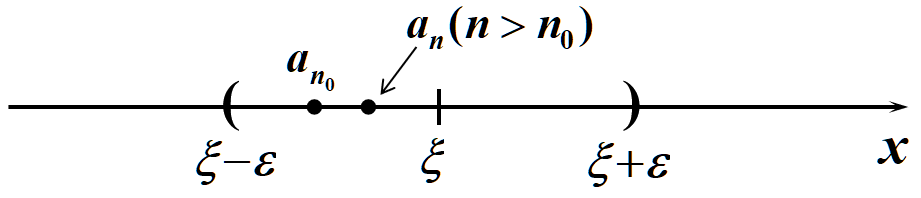
\includegraphics[width=0.5\textwidth]{figures/ddyoujie1.png}
% \caption{~}
\vspace{-0.85\baselineskip}
\end{wrapfigure}

$$
\xi-\varepsilon<a_{n_0} \leq a_n \leq \xi<\xi+\varepsilon,
$$
这就证明了 $\lim _{n \rightarrow \infty} a_n=\xi$.


\end{frame}

\begin{frame}{}%%%%
\begin{ex}
    设 $a_1=\sqrt{2}, \cdots, a_n=\underbrace{\sqrt{2+\sqrt{2+\cdots+\sqrt{2}}}}_n, \cdots$, 求 $\lim _{n \rightarrow \infty} a_n$. 
\end{ex}
\jie 显然 $a_n>0$. 因 $a_2=\sqrt{2+\sqrt{2}}$, 故 $a_2>a_1$; 设 $a_n>a_{n-1}$, 则有
$$
\begin{aligned}
a_{n+1}-a_n & =\sqrt{2+a_n}-\sqrt{2+a_{n-1}} \\
& =\frac{a_n-a_{n-1}}{\sqrt{2+a_n}+\sqrt{2+a_{n-1}}}>0,
\end{aligned}
$$
所以 $\left\{a_n\right\}$ 递增. 下面再来证明此数列有上界.
显然, $a_1=\sqrt{2}<2$, 设 $a_n<2$, 则
$$
a_{n+1}=\sqrt{2+a_n}<\sqrt{2+2}=2 .
$$
由此得到 $\left\{a_n\right\}$ 有上界 2 , 故极限 $\lim _{n \rightarrow \infty} a_n=A$ 存在.

\end{frame}
\begin{frame}{}%%%%
  于是由 $\lim _{n \rightarrow \infty} a_{n+1}=\lim _{n \rightarrow \infty} \sqrt{2+a_n}$, 可得\\
$A^2=2+A$, 并解出 $A=2, A=-1$.\\
由极限的不等式性, 知道 $A>0$, 所以
$$
\lim _{n \rightarrow \infty} a_n=2 \text {. }
$$  
\begin{ex}
下面的叙述错在哪儿?
\end{ex}
“设 $a_n=2^n, n=1,2, \cdots$, 则
$$
a_{n+1}=2^{n+1}=2 a_n .
$$
因为显然有 $a_n>0$, 所以 $\left\{a_n\right\}$ 递增. 设 $\lim _{n \rightarrow \infty} a_n=A$, 从而得出
$$
A=2 A \Rightarrow A=0
$$
即 $\lim _{n \rightarrow \infty} 2^n=0$."

\end{frame}

\begin{frame}{}%%%%
 以前知道圆周率 $\pi$ 是一个重要的无理数, 现在来 介绍另一个重要的无理数 $\re$.   \\
 考察数列 $\left\{e_n\right\}=\left\{\left(1+\frac{1}{n}\right)^n\right\}$ 的收敛性, 下面的证法 是最基本的,而教材上的证法技巧性较强. 利用二项式展开, 得
 \vskip 0.3\baselineskip
 \bena
$$
\begin{aligned}
e_n= & 1+n \frac{1}{n}+\frac{n(n-1)}{2 !} \frac{1}{n^2}+\cdots+\frac{n(n-1) \cdots 1}{n !} \frac{1}{n^n} \\
= & +\frac{1}{1 !}+\frac{1}{2 !}\left(1-\frac{1}{n}\right)+\frac{1}{3 !}\left(1-\frac{1}{n}\right)\left(1-\frac{2}{n}\right) \\
& +\cdots+\frac{1}{n !}\left(1-\frac{1}{n}\right)\left(1-\frac{2}{n}\right) \cdots\left(1-\frac{n-1}{n}\right),
\end{aligned}
$$
\eena
 由此得
\end{frame}

\begin{frame}{}%%%%

$$
\begin{aligned}
e_{n+1}=1 & +\frac{1}{1 !}+\frac{1}{2 !}\left(1-\frac{1}{n+1}\right)+\frac{1}{3 !}\left(1-\frac{1}{n+1}\right)\left(1-\frac{2}{n+1}\right) \\
& +\cdots+\frac{1}{n !}\left(1-\frac{1}{n+1}\right)\left(1-\frac{2}{n+1}\right) \cdots\left(1-\frac{n-1}{n+1}\right) \\
& +\frac{1}{(n+1) !}\left(1-\frac{1}{n+1}\right)\left(1-\frac{2}{n+1}\right) \cdots\left(1-\frac{n}{n+1}\right) .
\end{aligned}
$$
\vsp
把 $e_n$ 和 $e_{n+1}$ 的展开式作比较就可发现, $e_n$ 的展开 式有 $n+1$ 项, 其中的每一项都比 $e_{n+1}$ 的展开式中 的前 $n+1$ 项小, 而 $e_{n+1}$ 的最后一项大于零. 因此  
$$
e_n<e_{n+1}, \quad n=1,2, \cdots,
$$
从而 $\left\{\mathrm{e}_n\right\}$ 是单调增数列, 且

\end{frame}

\begin{frame}{}%%%%
  \bena
e_n \leqslant 1+\frac{1}{1 !}+\frac{1}{2 !}+\frac{1}{3 !}+\cdots+\frac{1}{n !} .
\eena
由此 $e_n \leq 1+1+\frac{1}{2}+\frac{1}{2^2}+\cdots+\frac{1}{2^{n-1}}<3$, 这就证明了 $\left\{e_n\right\}$ 又是有界数列. 于是 $\lim _{n \rightarrow \infty} e_n$ 存在. 记此极限为 $\mathbf{e}$, 即
\liang{
$$
\mathrm{e}=\lim _{n \rightarrow \infty}\left(1+\frac{1}{n}\right)^n.
$$ } 
\end{frame}

\begin{frame}{}%%%%
\setcounter{starli}{2}
\begin{starli}
 设 $s_n=1+\frac{1}{1 !}+\frac{1}{2 !}+\frac{1}{3 !}+\cdots+\frac{1}{n !}, n=1,2, \cdots$, 证明:
$$
\lim _{n \rightarrow \infty} s_n=\mathrm{e} .
$$ 
\end{starli}
\zheng 显然 $\left\{s_n\right\}$ 是单调增数列, 且由例 2 中的 (2) 式,
$$
\begin{aligned}
e_n & \leq 1+\frac{1}{1 !}+\frac{1}{2 !}+\frac{1}{3 !}+\cdots+\frac{1}{n !} \\
& =s_n<1+1+\frac{1}{2}+\frac{1}{2^2}+\cdots+\frac{1}{2^{n-1}}<3,
\end{aligned}
$$\vsp
因此 $\lim _{n \rightarrow \infty} s_n$ 存在且由极限的保不等式性,
$$
\mathrm{e}=\lim _{n \rightarrow \infty} e_n \leq \lim _{n \rightarrow \infty} s_n \text {. }
$$  
\end{frame}

\begin{frame}{}%%%%
    又对任意 $\boldsymbol{n}>\boldsymbol{m}$ ,
$$
\begin{aligned}
e_n=1 & +\frac{1}{1 !}+\frac{1}{2 !}\left(1-\frac{1}{n}\right)+\frac{1}{3 !}\left(1-\frac{1}{n}\right)\left(1-\frac{2}{n}\right) \\
& +\cdots+\frac{1}{n !}\left(1-\frac{1}{n}\right)\left(1-\frac{2}{n}\right) \cdots\left(1-\frac{n-1}{n}\right) \\
>1 & +\frac{1}{1 !}+\frac{1}{2 !}\left(1-\frac{1}{n}\right)+\frac{1}{3 !}\left(1-\frac{1}{n}\right)\left(1-\frac{2}{n}\right) \\
& +\cdots+\frac{1}{m !}\left(1-\frac{1}{n}\right)\left(1-\frac{2}{n}\right) \cdots\left(1-\frac{m-1}{n}\right),
\end{aligned}
$$
因此, 在上式中两边令 $n \rightarrow \infty$, 得
$$
\mathrm{e}=\lim _{n \rightarrow \infty} e_n \geq 1+\frac{1}{1 !}+\frac{1}{2 !}+\frac{1}{3 !}+\cdots+\frac{1}{m !}=s_m .
$$
当 $m \rightarrow \infty$ 时,由极限的保不等式性, $\mathrm{e} \geq \lim _{m \rightarrow \infty} s_m$.
从而
$$
\mathrm{e}=\lim _{n \rightarrow \infty} s_n=\lim _{n \rightarrow \infty}\left(1+\frac{1}{1 !}+\frac{1}{2 !}+\frac{1}{3 !}+\cdots+\frac{1}{n !}\right) .
$$

\end{frame}

\begin{frame}{}%%%%
  由公式 $\mathrm{e}=\lim _{n \rightarrow \infty}\left(1+\frac{1}{1 !}+\frac{1}{2 !}+\frac{1}{3 !}+\cdots+\frac{1}{n !}\right)$, 可以较快 地算出 $\mathrm{e}$ 的近似值.  \\
  由于
$$
0<s_{n+m}-s_n=\frac{1}{(n+1) !}+\frac{1}{(n+2) !}+\cdots+\frac{1}{(n+m) !},
$$
令 $\boldsymbol{m} \rightarrow \infty$, 得到
$$
0<e-s_n \leq \frac{1}{n ! n}, n=1,2, \cdots .
$$
取 $n=10, \mathrm{e} \approx s_{10} \approx 2.7182818$, 其误差
$$
0<\mathrm{e}-s_{10} \leq \frac{1}{10 \cdot 10 !}<10^{-7}.
$$
\end{frame}

\begin{frame}{}%%%%
\addtocounter{ex}{1}
\begin{ex}
   设 $S$ 是有界数集. 证明: 若 $\sup S=a \notin S$, 则存 在严格单调增数列 $\left\{x_n\right\} \subset S$, 使得 $\lim _{n \rightarrow \infty} x_n=a$. 
\end{ex}
\zheng 因 $a$ 是 $S$ 的上界, 故对 $\forall \varepsilon>0, \exists x \in S$, 使得 $\boldsymbol{x}>\boldsymbol{a}-\varepsilon$. 又因 $a \notin \boldsymbol{S}$, 故 $\boldsymbol{x}<\boldsymbol{a}$, 从而有
$$
\boldsymbol{a}-\varepsilon<\boldsymbol{x}<\boldsymbol{a} .
$$
现取 $\varepsilon_1=1$, 则 $\exists x_1 \in S$, 使得
$$
a-\varepsilon_1<x_1<a .
$$
再取 $\varepsilon_2=\min \left\{\frac{1}{2}, a-x_1\right\}$, 则 $\exists x_2 \in S$, 使得  
$$
a-\varepsilon_1<x_2<a,
$$

\end{frame}
\begin{frame}{}%%%%
  且有 $x_2>a-\varepsilon_2 \geq a-\left(a-x_1\right)=x_1$.
一般地,按上述步骤得到 $\boldsymbol{x}_{n-1}$ 之后, 取
$$
\varepsilon_n=\min \left\{\frac{1}{n}, a-x_{n-1}\right\},
$$
则存在 $x_n \in S$,使得
$$
a-\varepsilon_n<\boldsymbol{x}_n<a
$$
且有 $x_n>a-\varepsilon_n \geq a-\left(a-x_{n-1}\right)=x_{n-1}$.
于是得到 $\left\{x_n\right\} \subset S$, 它是严格单调的, 满足  
$$
a-\varepsilon_n<\boldsymbol{x}_n<\boldsymbol{a},
$$
因此, $\left|x_n-a\right|<\varepsilon_n \leq \frac{1}{n}, n=1,2, \cdots$.
这就证明了 $\lim _{n \rightarrow \infty} x_n=a$.
\end{frame}

\begin{frame}{二、柯西收敛准则}%%%%
\begin{thm}
 数列 $\left\{a_n\right\}$ 收敛的充要条件是:
对于任意正数 $\varepsilon$, 存在 $N>0$, 当 $n, m>N$ 时, 有
$$
\left|a_n-a_m\right|<\varepsilon . 
$$
\end{thm}
柯西准则的充要条件可用另一种形式表达为:
$\forall \varepsilon>0, \exists N>0$, 当 $n>N$ 时, 对任意 $p \in \mathbf{N}_{+}$, 均有
$$
\left|a_n-a_{n+p}\right|<\varepsilon .
$$
满足上述条件的数列称为\liang{柯西列}.   
由于该定理充分性的证明需要进一步的知识, 因 此这里仅给出必要性的证明.

\end{frame}


\begin{frame}{}%%%%
\zheng 设 $\lim _{n \rightarrow \infty} a_n=A$. 由极限定义, $\forall \varepsilon>0$, $\exists N>0$, 当 $n, m>N($ 或 $n, m \geq N)$ 时, 有
$$
\left|a_n-A\right|<\frac{\varepsilon}{2},\quad \left|a_m-A\right|<\frac{\varepsilon}{2} . 
$$
由此推得
$$
\left|a_n-a_m\right| \leq\left|a_n-A\right|+\left|a_m-A\right|<\frac{\varepsilon}{2}+\frac{\varepsilon}{2}=\varepsilon .
$$  
\begin{wrapfigure}{l}{0.3\textwidth}
\vspace{-0.85\baselineskip}
% \renewcommand{\figurename}{图}
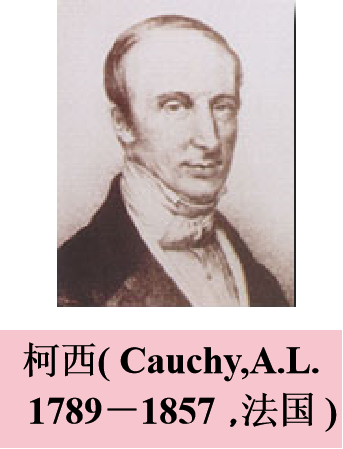
\includegraphics[width=0.3\textwidth]{figures/cauchy.png}
% \caption{~}
\vspace{-0.85\baselineskip}
\end{wrapfigure}
\end{frame}

\begin{frame}{}%%%%
\begin{ex}
    设 $x_n=1+\frac{1}{3}+\cdots+\frac{1}{n}, n=1,2, \cdots$. 证明 $\left\{x_n\right\}$ 发散.
\end{ex}
\zheng 取 $\varepsilon_0=\frac{1}{2}, \forall N>0, \exists n_0=N, m_0=2 N$, 使得
$$
\begin{aligned}
\left|x_{n_0}-x_{m_0}\right| & =\frac{1}{N+1}+\frac{1}{N+2}+\cdots+\frac{1}{2 N} \\
& \geq \frac{1}{2 N}+\frac{1}{2 N}+\cdots+\frac{1}{2 N} \geq \varepsilon_0 .
\end{aligned}
$$\vsp
由柯西收敛准则的否定陈述, 可知 $\left\{x_n\right\}$ 发散.    
\end{frame}

\begin{frame}{}%%%%
\begin{ex}
  设 $x_n=\frac{\sin 1}{2^1}+\frac{\sin 2}{2^2}+\cdots+\frac{\sin n}{2^n}, n=1,2, \cdots$. 求证 $\left\{x_n\right\}$ 收敛.  
\end{ex}
\zheng $\forall \varepsilon>0, \exists N=\frac{-\log \varepsilon}{\log 2}$, 当 $n>m>N$ 时, 有
$$
\begin{aligned}
\mid x_n- & x_m|=| \frac{\sin (m+1)}{2^{m+1}}+\cdots+\frac{\sin n}{2^n} \mid \\
& \leq \frac{1}{2^{m+1}}+\cdots+\frac{1}{2^n}=\frac{1}{2^{m+1}}\left(1+\frac{1}{2}+\cdots+\frac{1}{2^{n-m-1}}\right) \\
& =\frac{2}{2^{m+1}}\left(1-\frac{1}{2^{n-m}}\right) \leq \frac{1}{2^m}<\varepsilon \Rightarrow\left\{x_n\right\} \text { 收敛. }
\end{aligned}
$$ 
\end{frame}

\begin{frame}{}%%%%
\begin{ex}
 设数列满足条件: $\left|a_{n+1}-a_n\right|<r^n, n=1,2, \cdots$, 其中 $r \in(0,1)$. 求证 $\left\{a_n\right\}$ 收敛.
\end{ex}
\zheng 若 $n<m$, 则
$$
\begin{aligned}
\left|a_n-a_m\right| & \leq\left|a_n-a_{n+1}\right|+\left|a_{n+1}-a_{n+2}\right|+\cdots+\left|a_{m-1}-a_m\right| \\
& \leq r^n+r^{n+1}+\cdots+r^{m-1}=\frac{r^n-r^m}{1-r}<\frac{r^n}{1-r} .
\end{aligned}
$$
由于 $\lim _{n \rightarrow \infty} \frac{r^n}{1-r}=0$, 于是 $\forall \varepsilon>0, \exists N, n>N$,
$$
\left|\frac{r^n}{1-r}\right|<\varepsilon.
$$   
若 $\boldsymbol{m}>\boldsymbol{n}>\boldsymbol{N}$, 就有
$$
\left|\boldsymbol{a}_{\boldsymbol{n}}-\boldsymbol{a}_m\right| \leq\left|\frac{\boldsymbol{r}^n}{\mathbf{1 - r}}\right|<\varepsilon .
$$
由柯西准则, $\left\{\boldsymbol{a}_n\right\}$ 收敛.
\end{frame}
\begin{frame}{}%%%%
\zhu{柯西收敛准则的意义在于:可以根据数列通 项本身的特征来判断该数列是否收敛, 而不必依 赖于极限定义中的那个极限值 $\boldsymbol{A}$. 这一特点在理 论上特别有用, 大家将会逐渐体会到它的重要性.} 

\end{frame}

\begin{frame}{  复习思考题}%%%%
1. 对于数列是否收敛的各种判别法加以总结.\\
2. 试给出 $\left\{a_n\right\}$ 不是柯西列的正面陈述.    
\end{frame}

\end{document}


